\documentclass{article}
\usepackage[utf8]{inputenc}
\usepackage{ctex}
\usepackage{graphicx}
\usepackage{hyperref}
\usepackage[top=2.8cm,bottom=2.8cm,right=2.5cm,left=2.5cm]{geometry}
\usepackage{subfigure}
\usepackage{amsmath}
\usepackage{amssymb}
\usepackage{amsfonts}
\usepackage{ifthen}

\newcommand{\task}[1]{\noindent\textbf{Problem}:#1}
\newcommand{\question}[1]{\noindent?\emph{#1}}
\newcommand{\mathdef}[2]{\noindent \textbf{\underline{Def}} \quad\textbf{#1} #2}
\newcommand{\important}[1]{\noindent\textbf{\underline{#1}}\quad}

%notations -- must be used in equation environment!
\newcommand{\rms}[1]{E_{\mathrm{RMS}}(#1)}
\newcommand{\errorfunc}[1]{E(#1)}
\newcommand{\bestcoefvec}{\mathbf{w}_*}
\newcommand{\coefvec}{\mathbf{w}}
\newcommand{\numofdata}[1]{N_{#1}}

%terminologies -- must be used in equation environment
\newcommand{\maxlikelyhood}[1][]{%
    \ifthenelse{\equal{#1}{}}{极大似然(Maximum Likelyhood)}{极大似然}}
\newcommand{\lsr}[1][]{%
    \ifthenelse{\equal{#1}{full}}{最小二乘法(Least Square Root)}{%
    \ifthenelse{\equal{#1}{p}}{最小二乘原则}{最小二乘法}}}
\newcommand{\bayesian}[2][]{%
    \ifthenelse{\equal{#1}{full}}{贝叶斯( Bayesian)}{贝叶斯#2}
}
\newcommand{\regularization}[2][]{%
    \ifthenelse{\equal{#1}{full}}{正规化( Regularization)}{正规化#2}
}



\title{模式识别与机器学习\\Pattern Recognition and Machine Learning}
\author{Ding Zhang}
\date{March 2019}

\begin{document}

\maketitle

\section{入门、概率论、决策论及信息论}
\subsection{机器学习的知识框架}
    \begin{figure}[h]
        \centering
        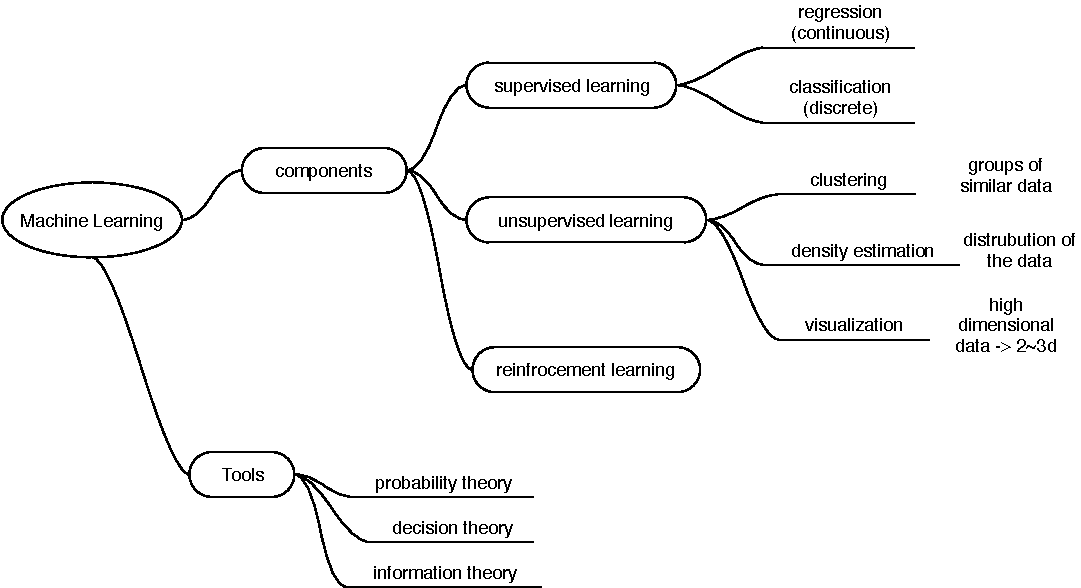
\includegraphics[width=\textwidth]{figures/pattern_recognition_machine_learning-outline.pdf}
        \caption{Outline of Machine Learning}
        \label{fig:outline}
    \end{figure}

\subsection{A regression example: Curve-Fitting}
\task{给定规模为$N$的数据集$\mathrm{dataset}=\{(x_i,t_i) | i=1,2,\cdots,N\}$,希望通过数据集找到$f:x\mapsto t$,对未知的$x$对应的$t$值进行预测}
    
    最朴素的想法就是进行\textbf{多项式拟合(Polynomial Fitting)},定义多项式\ref{polynomial}:
    \begin{equation}
        f(x,\mathbf{w})=w_0+w_1x+w_2x^2+\cdots+w_Mx^M
        \label{polynomial}
    \end{equation}
    多项式是关于\(\mathbf{w}\)的线性函数

\question{如何去寻找系数$\mathbf{w}$}

    我们定义一个误差函数如\ref{error_eqa}所示:
    \begin{equation}
        E(\textbf{w})=\frac{1}{2}\sum_{i=1}^{N}[f(x_i, \textbf{w})-t_i]^2
        \label{error_eqa}
    \end{equation}
    
    这是一个最优化问题,因为误差函数是关于系数的二次型,导数必然是线性的,对于一个确定的阶数$M$,一定存在一个最优解$\mathbf{w}_*$。
    
    需要注意$\mathbf{w}_*$和$M$是对应的,不同的阶数\(M\)对应着不同的模型复杂度,也对应着不同的\(\textbf{w}_*\)。
    在不同的模型(curve-fitting中的\(M\)的选择)之中作出抉择即\textbf{模型比较或模型选择(Model Comparison/Model Selection)}问题是机器学习中的一类重要问题
    
    \textbf{欠拟合(Under-fitting)与过拟合(Over-fitting)问题}: 在curve-fitting问题中,当选择的模型阶数过低,模型无法反映出数据真值的变化;
    当选择的模型的阶数过高时,尽管模型对数据集的误差非常小,但是多项式的系数会非常之大,造成严重的震荡。
    \begin{figure}[h]
        \centering
        \subfigure[不同复杂度(不同阶数)的模型的拟合效果]{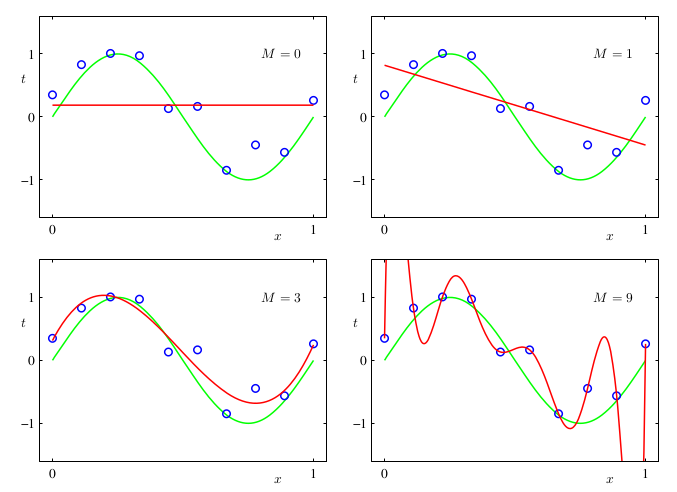
\includegraphics[width=.45\textwidth]{figures/polynomial_curve_fitting.png}}
        \quad
        \subfigure[$\rms{\bestcoefvec}$~$M$]{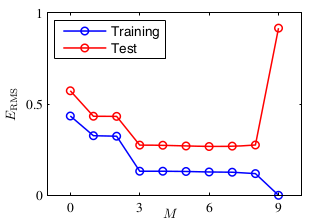
\includegraphics[width=.45\textwidth]{figures/e_rms.png}\label{fig:e_rms}}
        \caption{不同的模型之间的比较}
        \label{fig:polynomial_fitting}
    \end{figure}
    
    这里需要一个衡量拟合效果的标准,我们采用$N$个数据得到了模型$f(x,\mathbf{w}_*)$,当需要检测模型的效果时,可以测量得到更大的数据集,计规模为$N_{test}$,则测试集计算得到的误差函数为:$E(\mathbf{w}_*)$,为了比较不同阶数多项式的拟合效果,可以用\textbf{均方根值(Root Mean Square, RMS)}来进行比较:
    \begin{equation}
        \rms{\bestcoefvec}=\sqrt{2E(\bestcoefvec)/N_{test}}
        \label{eqa:rms}
    \end{equation}
    
    如图\ref{fig:polynomial_fitting}所示,当$N=10$时,$M$在超过9后($\coefvec_* \in \mathbb{R}^{10}$ ),拟合效果变差。当我们增加数据集的规模$N$,$M=9$的拟合效果会慢慢变好。
    
    对$\errorfunc{\coefvec}$的最优化问题本质即是\textbf{\lsr[full]},而最小二乘法是\textbf{\maxlikelyhood}的一个特例。可以看到\lsr 模型复杂度受到数据集大小的限制,而之后会介绍的\textbf{\bayesian[full]}则可以避免过拟合的发生,它对数据集的规模是自适应的。
    
    这里先暂时不介绍\bayesian 的内容,而尝试将\lsr 方法进行优化,通过观察发现$M>N$造成的过拟合震荡主要源于异常大的系数,这里考虑在$E(\coefvec)$中加入惩罚项(Penalty Term),再对新的目标函数进行最优化,从而来避开$\|\coefvec_*\|$过大的求解域,这一过程称之为\textbf{\regularization[full]}
    \begin{equation}
        \Tilde{E}(\coefvec)=\frac{1}{2}\sum_{i=1}^N[f(x_i, \coefvec)-t_i]^2 + \frac{\lambda}{2} \coefvec^T\coefvec \footnote{$\omega_0^2$常常省略,具体5.5.1会讲到}, \lambda \geq 0 
        \label{eqa:regularization}
    \end{equation}
    
    这种正规划方法在不同的领域有不同的名称,在统计学领域,因为它能将系数缩小,称之为\textbf{Shrinkage};这个特殊的正规项也称\textbf{ridge regression};在神经网络中,这种方法叫做\textbf{权重衰减(Weight Decay)}

\subsection{概率论}
    概率论是我们用来度量不确定度(Uncertainty)的理论工具,其中包括不确定度的量化(quantification)以及操作(Manipulation)。概率论和之后介绍的决策论将共同形成一套最优预测的方案(Optimal Prediction)。
    \subsubsection{基础概念及重要性质}
    \mathdef{Probability}{of an event  is the fraction of times that event occurs out of total number of trials, in the limit the total number of trials goes to infinity.}
    \begin{figure}[h]
        \centering
        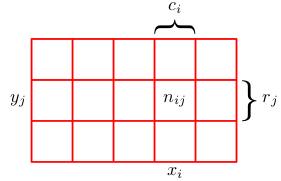
\includegraphics[width=.4\linewidth]{figures/prob_concepts.png}
        \caption{两个随机变量$X$与$Y$}
        \label{fig:prob_concepts}
    \end{figure}
    
    \important{常见的几个概率}
    \begin{description}
        \item[概率] 
        $p(X=x_i, Y=y_j)=\frac{n_{ij}}{N}$
        
        \item[边缘概率(Marginal Probability)]
        $p(X=x_i)=p(X=x_i,Y)=\frac{c_i}{N}$
        
        $p(x_i)=\int_{-\infty}^{+\infty}{p(x_i,y)}\,\mathrm{d}y$
        
        \item[条件概率(Conditional Probability)]
        $p(X=x_i|Y=y_j)=\frac{n_{ij}}{r_j}=\frac{n_{ij}/{N}}{r_j/N}=\frac{p(X=x_i, Y=y_j)}{p(Y=y_j)}$
        
        probability of A given B:
        \[p(A|B)=\frac{p(AB)}{p(B)}\]
    \end{description}
    
    \important{两条重要规则}
    
        加法规则(sum rule):
        $p(X)=\sum_Yp(X,Y)$
        
        乘法规则(product rule):
        $p(X)=p(XY)/p(Y|X)$
        
    \subsubsection{\bayesian[full]}
    基于先验信息的概率计算问题
        \begin{align*}
            p(X|Y) & = \frac{p(XY)}{p(Y)}\\
                &= \frac{p(Y|X)p(X)}{p(Y)} 
        \end{align*}
    
    在$Y$发生的条件下,$X$的概率。这里$p(X)$称之为先验概率(Prior Probability),它是基于历史观测和经验得到的;$p(X|Y)$称之为后验概率(Posterior Probability),该概率是对Y的观测完成之后才得到的,可以通过\bayesian{定理}得到。
    
    \subsubsection{概率密度}
    
\end{document}
